\documentclass[fontsize=11pt]{article}
\usepackage{amsmath}
\usepackage{graphicx}
\usepackage[utf8]{inputenc}
\usepackage[margin=0.75in]{geometry}

\title{CSC110 Project Proposal: An Investigation of the Political Satisfaction of the General Public over the COVID-19 Pandemic}
\author{Aviraj Newatia, Mishaal Kandapath, Rudraksh Monga, Taylor Whatley}
\date{Friday, November 5, 2021}

\begin{document}
\maketitle

\section*{Problem Description and Research Question}

TODO

\section*{Dataset Description}

The dataset we will be using was sourced from the online machine learning data repository Kaggle, a subsidiary of Google LLC, which serves as an online community of data scientists and machine learning practitioners. 
\\\\
It is a csv (comma-separated values) file of 17,777,472 unique comments related to covid that were collated from the online forum platform Reddit. The dataset is called The Reddit COVID dataset [https://www.kaggle.com/pavellexyr/the-reddit-covid-dataset].
\\\\
We transformed this dataset by filtering by the subreddit the comment came from, building a sub-dataset of comments only from political subreddits such as r/uspolitics. 
\\\\
The dataset was too large to load into Excel, so we filtered the first 2 million comments using pandas in Python to yield 32,335 comments. 
\\\\
The dataset has 10 columns, of which we extracted and will be using 2 which are the actual text of the comment ("body") and the timestamp of creation/posting ("created\_utc"). \\\\
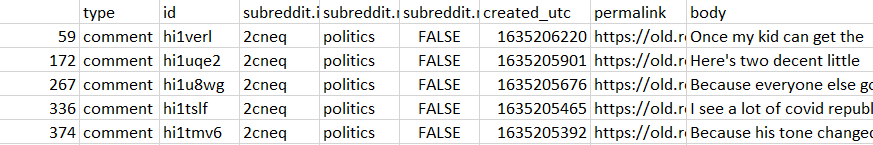
\includegraphics{rows.png}

\section*{Computational Plan}

TODO

\section*{References}

TODO

% NOTE: LaTeX does have a built-in way of generating references automatically,
% but it's a bit tricky to use so we STRONGLY recommend writing your references
% manually, using a standard academic format like APA or MLA.
% (E.g., https://owl.purdue.edu/owl/research_and_citation/apa_style/apa_formatting_and_style_guide/general_format.html)

\end{document}
